\documentclass[10pt,preprint]{aastex}

\usepackage{amsfonts}
\usepackage{amsmath}
\usepackage{amssymb}
\usepackage{amsthm}
\usepackage{booktabs}
\usepackage{mathrsfs}
\usepackage{cite}
\usepackage{times}
\usepackage{url}
\usepackage{hyperref}
\usepackage{lineno}
\usepackage{yhmath}
\usepackage{natbib}
\usepackage{../definitions}
\hypersetup{
  bookmarksnumbered = true,
  bookmarksopen=false,
  pdfborder=0 0 0,         % make all links invisible, so the pdf looks good when printed
  pdffitwindow=true,      % window fit to page when opened
  pdfnewwindow=true, % links in new window
  colorlinks=true,           % false: boxed links; true: colored links
  linkcolor=blue,            % color of internal links
  citecolor=magenta,    % color of links to bibliography
  filecolor=magenta,     % color of file links
  urlcolor=cyan              % color of external links
}

\usepackage{graphicx}
\newtheorem{remark}{Remark}
\graphicspath{{Figures/}}

\usepackage{float}

\begin{document}

\title{Nodal Discontinuous Galerkin Method for the Euler Equations in GR}
\author{Samuel J Dunham\altaffilmark{1}, Eirik Endeve\altaffilmark{2}, et al.}
\altaffiltext{1}{Department of Astronomy, Vanderbilt University, 6301 Stevenson Science Center, Nashville TN, 37212, USA; samuel.j.dunham@vanderbilt.edu}
\altaffiltext{2}{Computational and Applied Mathematics Group, Oak Ridge National Laboratory, Oak Ridge, TN 37831-6354, USA; endevee@ornl.gov}

\tableofcontents

\section{Discontinuous Galerkin Scheme}
\label{sec:dgMethod}

We assume a spacetime metric
\begin{equation}
  ds^{2}=-\alpha^{2}\,dt^{2}+\gamma_{ij}\,dx^{i}\,dx^{j},
\end{equation}
and consider the system of conservation laws with sources
\begin{equation}
  \pd{}{t}\big(\sqrt{\gamma}\,\bU\big)+\sum_{i=1}^{d}\pd{}{i}\big(\alpha\,\sqrt{\gamma}\,\bF^{i}(\bU)\big)=\alpha\,\sqrt{\gamma}\,\bG(\bU),
  \label{eq:conservationLaws}
\end{equation}
where
\begin{align}
  \bU
  &=\big(D,\,S_{j},\,\tau\big)^{\mbox{\tiny T}}
  =\big(\rho\,W,\,\rho\,h\,W^{2}\,v_{j},\,\rho\,W\left(h\,W-1\right)-p\big)^{\mbox{\tiny T}}, \\
  \bF^{i}(\bU)
  &=\big(D\,v^{i},\,\big)^{\mbox{\tiny T}}
\end{align}
\newpage

\section{Bound-Preserving Methods Using First-Order DG Scheme}

\subsection{Cartesian Coordinates}
This section closely follows \citet{Qin2016}.

\subsubsection{Set of Admissible States}
We consider a one-dimensional system of conservation laws:
\begin{equation}
    \pd{\,\bU}{t} + \pd{\,\bF\left(\bU\right)}{x} = \vect{0},
\end{equation}
where $\bU$ is a vector of conserved variables, defined as:
\begin{equation}\label{Eq:ConservedVariables}
    \bU\longrightarrow\begin{pmatrix} D\\ S\\ \tau\end{pmatrix}=\begin{pmatrix} \rho\,W\\ \rho\,h\,W^{2}\,v\\ \rho\,W\left(h\,W-1\right)-p\end{pmatrix},
\end{equation}
and $\bF\left(\bU\right)$ are the fluxes of those conserved quantities:
\begin{equation}\label{Eq:FluxVector}
    \bF\left(\bU\right)\longrightarrow\begin{pmatrix}\rho\,W\,v\\ \rho\,h\,W^{2}\,v^{2}+p\\\rho\,h\,W^{2}\,v-D\,v\end{pmatrix}.
\end{equation}


The physics leads us to define a set of admissible states, $\cG_{p}$ (the subscript $p$ stands for primitive), as:
\begin{equation}
    \cG_{p}\equiv\left\{\bU\Big|\rho>0,\,p>0,\,v^{2}<1\right\}.
\end{equation}

It is shown in \citet{Mignone2005} that $\cG$ is a convex set\footnote{Convex in the sense that if $\bU_{1}\in\cG$ and $\bU_{2}\in\cG$, then $\alpha_{1}\,\bU_{1}+\alpha_{2}\,\bU_{2}\in\cG$, where $\alpha_{1},\,\alpha_{2}\in\left[0,1\right]$ and $\alpha_{1}+\alpha_{2}=1$.} and can equivalently be written in terms of the conserved variables as:
\begin{equation}\label{Eq:SetOfAdmissibleStates}
    \cG\equiv\left\{\bU\Big|D>0,\,\tau+D>\sqrt{D^{2}+S^{2}}\right\}.
\end{equation}

\subsubsection{Time-Step Derivation/CFL Condition}
For the first-order DG method using forward-Euler time-stepping, we evolve the vector of conserved variables as:
\begin{equation}\label{Eq:1stOrderDG}
    \ol{\bU}^{n+1}_{i}=\ol{\bU}^{n}_{i}-\eta_{i}\left[\hat{\bF}\left(\ol{\bU}^{n}_{i},\ol{\bU}^{n}_{i+1}\right)-\hat{\bF}\left(\ol{\bU}^{n}_{i-1},\ol{\bU}^{n}_{i}\right)\right],
\end{equation}
where
\begin{equation}
    \ol{\bU}_{i}\equiv\f{1}{\Delta x_{i}}\int_{x_{\imh}}^{x_{\iph}}\bU_{i}\,dx,
\end{equation}
$\eta_{i}\equiv\Delta t_{i}/\Delta x_{i}$, and $\hat{\bF}$ is the numerical flux. In this document we use the local Lax-Friedrichs flux, defined as:
\begin{equation}\label{Eq:LLF}
    \hat{\bF}\left(a,b\right)=\f{1}{2}\left[\bF\left(a\right)+\bF\left(b\right) - \alpha_{ab}\left(b-a\right)\right],
\end{equation}
where $a$ and $b$ represent the state of the fluid in two different elements, $\alpha_{ab}$ is an estimate for the wave-speed:
\begin{equation}
    \alpha_{ab}=\text{max}\left[\alpha\left(a\right),\alpha\left(b\right)\right],
\end{equation}
and $\alpha$ is the largest (in absolute value) eigenvalue of the flux-Jacobian:
\begin{equation}
    \alpha=\left|\left|\pderiv{\bF}{\bU}\right|\right|.
\end{equation}
Using this we define the following variables:
\begin{equation}\label{Eq:EigVals}
    \alpha_{\iph}=\text{max}\left[\alpha\left(\ol{\bU}_{i}\right),\alpha\left(\ol{\bU}_{i+1}\right)\right],\hspace{3em} \alpha_{\imh}=\text{max}\left[\alpha\left(\ol{\bU}_{i-1}\right),\alpha\left(\ol{\bU}_{i}\right)\right].
\end{equation}

Substituting \eqref{Eq:LLF} with \eqref{Eq:EigVals} into \eqref{Eq:1stOrderDG}:
\begin{align}
    \ol{\bU}^{n+1}_{i}&=\ol{\bU}^{n}_{i}-\f{\eta_{i}}{2}\left[\bF\left(\ol{\bU}^{n}_{i}\right)+\bF\left(\ol{\bU}^{n}_{i+1}\right)-\alpha_{\iph}\left(\ol{\bU}^{n}_{i+1}-\ol{\bU}^{n}_{i}\right)\right.\nonumber\\
    &\left.\hspace{7em}-\bF\left(\ol{\bU}^{n}_{i}\right)-\bF\left(\ol{\bU}^{n}_{i-1}\right)+\alpha_{\imh}\left(\ol{\bU}^{n}_{i}-\ol{\bU}^{n}_{i-1}\right)\right]\nonumber\\
    &=\left[1-\f{\eta_{i}}{2}\left(\alpha_{\iph}+\alpha_{\imh}\right)\right]\ol{\bU}^{n}_{i}+\f{\eta_{i}}{2}\,\alpha_{\iph}\left[\ol{\bU}^{n}_{i+1}-\f{1}{\alpha_{\iph}}\bF\left(\ol{\bU}^{n}_{i+1}\right)\right]\nonumber\\
    &\hspace{15em}+\f{\eta_{i}}{2}\,\alpha_{\imh}\left[\ol{\bU}^{n}_{i-1}+\f{1}{\alpha_{\imh}}\bF\left(\ol{\bU}^{n}_{i-1}\right)\right]\nonumber\\
    &=\left[1-\f{\eta_{i}}{2}\left(\alpha_{\iph}+\alpha_{\imh}\right)\right]\ol{\bU}^{n}_{i}+\f{\eta_{i}}{2}\,\alpha_{\iph}\,\ol{\bH}^{-}\left(\ol{\bU}^{n}_{i+1},\alpha_{\iph}\right)+\f{\eta_{i}}{2}\,\alpha_{\iph}\,\ol{\bH}^{+}\left(\ol{\bU}^{n}_{i-1},\alpha_{\imh}\right),\label{Eq:ConvComb}
\end{align}
where
\begin{equation}\label{Eq:Hpm}
    \ol{\bH}^{\pm}\left(\ol{\bU},\alpha\right)\equiv\ol{\bU}\pm\f{1}{\alpha}\,\bF\left(\ol{\bU}\right).
\end{equation}

The proof that $\ol{\bH}^{\pm}\in\cG$ is given in \citet{Qin2016}. Therefore, we see that with a restriction on $\alpha_{i\pm\f{1}{2}}$ that \eqref{Eq:ConvComb} is a convex combination. The restriction is (recalling that $\eta_{i}=\Delta t_{i}/\Delta x_{i}$):
\begin{equation}
    1-\f{\eta_{i}}{2}\left(\alpha_{\iph}+\alpha_{\imh}\right)>0\implies\f{\eta_{i}}{2}\left(\alpha_{\iph}+\alpha_{\imh}\right)<1\implies \Delta t_{i}<\f{2\,\Delta x_{i}}{\alpha_{\iph}+\alpha_{\imh}}\leq\f{\Delta x_{i}}{\text{max}\left(\alpha_{i\pm\f{1}{2}}\right)}.
\end{equation}

We want a time-step that is the same for all elements at a given time, so we tighten the restriction to:
\begin{equation}
    \Delta t<\text{min}_{i}\left(\f{\Delta x_{i}}{\text{max}\left(\alpha_{i\pm\f{1}{2}}\right)}\right)=\f{\Delta x}{\text{max}_{i}\left(\alpha_{i\pm\f{1}{2}}\right)},
\end{equation}
where the equality follows for a uniform mesh, i.e. $\Delta x_{i}=\Delta x\,\forall i$.

\newpage


\subsection{Curvilinear Coordinates in 1-D}
NOTE: We assume a conformally-flat, time-independent spatial three-metric:
\begin{equation}
    \gamma_{ij}\left(x^{k},t\right)\longrightarrow\psi^{4}\left(x^{k}\right)\,\ol{\gamma_{ii}}\left(x^{k}\right),
\end{equation}
where $\psi\left(x^{k}\right)$ is the conformal factor and $\ol{\gamma}_{ii}$ is the flat-space metric.

\subsubsection{Set of Admissible States}
We again consider a one-dimensional system of conservation laws, but this time with a curvilinear metric:
\begin{equation}\label{Eq:1DCurvilinearConsLaw}
    \pd{\left(\sqrtgm\,\bU\right)}{t}+\pd{\left(\sqrtgm\,\bF^{i}\right)}{i}=\sqrtgm\,\bQ,\hspace{1em}\text{(no sum on $i$)},
\end{equation}
where $\bU$ is given by:
\begin{equation}
    \bU\longrightarrow\begin{pmatrix} D\\ S_{j}\\ \tau\end{pmatrix}=\begin{pmatrix} \rho\,W\\ \rho\,h\,W^{2}\,v_{j}\\ \rho\,W\left(h\,W-1\right)-p\end{pmatrix}=\begin{pmatrix} \rho\,W\\ \rho\,h\,W^{2}\,\gamma_{jk}\,v^{k}\\ \rho\,W\left(h\,W-1\right)-p\end{pmatrix},
\end{equation}
$\bF^{i}\left(\bU\right)$ are the fluxes in the $x^{i}$-direction of those conserved quantities:
\begin{equation}
    \bF^{i}\left(\bU\right)\longrightarrow\begin{pmatrix}D\,v^{i}\\ S^{i}\,v_{j}+p\,\delta^{i}_{~j}\\ S^{i}-D\,v^{i}\end{pmatrix}=\begin{pmatrix}\rho\,W\,v^{i}\\ \rho\,h\,W^{2}\,v^{i}\,v_{j}+p\,\delta^{i}_{~j}\\\rho\,h\,W^{2}\,v^{i}-D\,v^{i}\end{pmatrix}=\begin{pmatrix}\rho\,W\,v^{i}\\ \rho\,h\,W^{2}\,\gamma_{jk}\,v^{i}\,v^{k}+p\,\delta^{i}_{~j}\\\rho\,h\,W^{2}\,v^{i}-D\,v^{i}\end{pmatrix},
\end{equation}
and $\bQ$ is a source term:
\begin{align}
    \bQ\longrightarrow\begin{pmatrix}0\\\f{1}{2}\,P^{ik}\,\pd{\,\gamma_{ik}}{j}\\0\end{pmatrix}&=\begin{pmatrix}0\\ \f{1}{2}\left[P^{11}\,\pd{\,\gamma_{11}}{j}+P^{22}\,\pd{\,\gamma_{22}}{j}+P^{33}\,\pd{\,\gamma_{33}}{j}\right] \\0\end{pmatrix}\\
    &=\begin{pmatrix}0\\ P^{11}\,h_{1}\,\pd{\,h_{1}}{j}+P^{22}\,h_{2}\,\pd{\,h_{2}}{j}+P^{33}\,h_{3}\,\pd{\,h_{3}}{j} \\0\end{pmatrix},
\end{align}
where we have used the fact that $\gamma_{kk}=\left(h_{k}\right)^{2}$. The $P^{ik}$ are components of the pressure tensor:
\begin{equation}
    P^{ik}=S^{i}\,v^{k}+p\,\gamma^{ik}=\gamma^{i\ell}\,S_{\ell}\,v^{k}+p\,\gamma^{ik}=\gamma^{i\ell}\,S_{\ell}\,v^{k}+p\,\gamma^{i\ell}\,\delta^{k}_{~\ell}=\gamma^{i\ell}\left(S_{\ell}\,v^{k}+p\,\delta^{k}_{~\ell}\right).
\end{equation}
Since the spatial three-metric is diagonal the only non-zero term is that with $\ell=i$. We can therefore simplify further:
\begin{equation}
    P^{ik}=\gamma^{ii}\left(S_{i}\,v^{k}+p\,\delta^{k}_{~i}\right)=\f{1}{\gamma_{ii}}\,\left(S_{i}\,v^{k}+p\,\delta^{k}_{~i}\right),\hspace{1em}\text{(no sum on $i$)}.
\end{equation}
For the source-term sum we then have:
\begin{equation}\label{Eq:PressureTensorSum}
    Q_{j}=\f{1}{2}\,P^{ik}\,\p_{j}\,\gamma_{ik}=\f{1}{2}\,P^{kk}\,\p_{j}\,\gamma_{kk}=\f{1}{2}\,P^{kk}\,\p_{j}\left(h_{k}\right)^{2}=P^{kk}\,h_{k}\,\p_{j}\,h_{k}.
\end{equation}

These definitions lead us to define the same set of admissible states as before, namely:
\begin{equation}
    \cG_{p}\equiv\left\{\bU\Big|\rho>0,\,p>0,\,v^{2}<1\right\},
\end{equation}
the only difference being that $v^{2}$ now involves the metric:
\begin{equation}
    v^{2}=v^{j}\,v_{j}=\gamma_{kj}\,v^{k}\,v^{j}.
\end{equation}

Before continuing, we show that the introduction of the metric doesn't affect the translation between $\cG_{p}$ and $\cG$...\sd{I've shown this, just need to TeX it up}

\subsubsection{Time-Step Derivation/CFL Condition}
We start by integrating both sides of \eqref{Eq:1DCurvilinearConsLaw} over $dx^{i}$ and dividing by the volume of the $K^{th}$ element, $\Delta V_{K}$ (recalling that there is no sum on $i$):
\begin{equation}
    \f{1}{\Delta V_{K}}\int_{x^{i}_{L}}^{x^{i}_{H}}\pd{\left(\sqrtgm\,\bU\right)}{t}dx^{i}+\f{1}{\Delta V_{K}}\int_{x^{i}_{L}}^{x^{i}_{H}}\pd{\left(\sqrtgm\,\bF^{i}\left(\bU\right)\right)}{i}dx^{i}=\f{1}{\Delta V_{K}}\int_{x^{i}_{L}}^{x^{i}_{H}}\sqrtgm\,\bQ\,dx^{i},
\end{equation}
where:
\begin{equation}
    \Delta V_{K}=\int_{x^{i}_{L}}^{x^{i}_{H}}dV=\int_{x^{i}_{L}}^{x^{i}_{H}}\sqrtgm\,dx^{i}.
\end{equation}

By defining the cell-average as:
\begin{equation}
    \bW_{K}\equiv\f{1}{\Delta V_{K}}\int_{x^{i}_{L}}^{x^{i}_{H}}\bW\,dV,
\end{equation}
we have:
\begin{equation}
    \f{d\,\bU_{K}}{dt}+\f{1}{\Delta V_{K}}\left.\left(\sqrtgm\,\hat{\bF}\left(\bU\right)\right)\right|^{x^{i}_{H}}_{x^{i}_{L}}=\bQ_{K}.
\end{equation}
Now, using the common notation of the time step being represented as a superscript $n$:
\begin{equation}
    \bU^{n+1}_{K}=\bU^{n}_{K}-\f{\Delta t^{n}_{K}}{\Delta V_{K}}\left[\sqrtgm_{H}\,\hat{\bF}^{n}_{H}-\sqrtgm_{L}\,\hat{\bF}^{n}_{L}\right]+\Delta t^{n}_{K}\,\bQ^{n}_{K}.
\end{equation}

Now we define a parameter a la \citet{ZS2011b}: $\ve\in\left(0,1\right)$, such that (NOTE: \citet{ZS2011b} set $\ve=1/2$):
\begin{equation}
    \bU^{n}_{K}=\ve\,\bU^{n}_{K}+\left(1-\ve\right)\bU^{n}_{K}.
\end{equation}
We can use the first term to balance out the term in the square brackets and the second term to balance out the source term.

So, we get:
\begin{align}
    \bU^{n+1}_{K}&=\ve\left\{\bU^{n}_{K}-\f{\Delta t^{n}_{K}}{\ve\,\Delta V_{K}}\left[\sqrtgm_{H}\,\hat{\bF}^{n}_{H}-\sqrtgm_{L}\,\hat{\bF}^{n}_{L}\right]\right\}+\left(1-\ve\right)\bU^{n}_{K}+\Delta t^{n}_{K}\,\bQ^{n}_{K}\\
    &=\ve\left\{\bU^{n}_{K}-\eta^{n}_{K}\left[\sqrtgm_{H}\,\hat{\bF}\left(\bU^{n}_{K+1},\bU^{n}_{K}\right)-\sqrtgm_{L}\,\hat{\bF}\left(\bU^{n}_{K},\bU^{n}_{K-1}\right)\right]\right\}+\left(1-\ve\right)\bU^{n}_{K}+\Delta t^{n}_{K}\,\bQ^{n}_{K}\\
    &=\ve\,\bH_{K,1}+\left(1-\ve\right)\bH_{K,2},
\end{align}
where
\begin{equation}
    \bH_{K,1}\equiv \bU^{n}_{K}-\eta^{n}_{K}\left[\sqrtgm_{H}\,\hat{\bF}\left(\bU^{n}_{K+1},\bU^{n}_{K}\right)-\sqrtgm_{L}\,\hat{\bF}\left(\bU^{n}_{K},\bU^{n}_{K-1}\right)\right],
\end{equation}
\begin{equation}
    \bH_{K,2}\equiv\bU^{n}_{K}+\f{\Delta t^{n}_{K}}{1-\ve}\,\bQ^{n}_{K},
\end{equation}
and
\begin{equation}
    \eta^{n}_{K}\equiv\f{\Delta t^{n}_{K}}{\ve\,\Delta V_{K}}.
\end{equation}

We proceed by focusing on each term individually, starting with the numerical flux term, $\bH_{K,1}$.

\subsubsection{Numerical flux term}
We have to show that $\bH_{K,1}\in\cG$. We again we use the Local-Lax-Friedrichs flux, \eqref{Eq:LLF}, yielding for $\bH_{K,1}$:
\begin{align}
    \bU^{n}_{K}-\f{\eta^{n}_{K}}{2}\Big\{&\sqrtgm_{H}\left[\bF\left(\bU^{n}_{K+1}\right)+\bF\left(\bU^{n}_{K}\right)-\alpha^{n}_{H}\left(\bU^{n}_{K+1}-\bU^{n}_{K}\right)\right]\\
    &-\sqrtgm_{L}\left[\bF\left(\bU^{n}_{K}\right)+\bF\left(\bU^{n}_{K-1}\right)-\alpha^{n}_{L}\left(\bU^{n}_{K}-\bU^{n}_{K-1}\right)\right]\Big\}\\
    &\hspace{-10em}=\left(1-\f{1}{2}\,\eta^{n}_{K}\,\sqrtgm_{H}\,\alpha^{n}_{H}-\f{1}{2}\,\eta^{n}_{K}\,\sqrtgm_{L}\,\alpha^{n}_{L}\right)\bU^{n}_{K}\\
    &\hspace{-8em}-\f{1}{2}\,\eta^{n}_{K}\,\sqrtgm_{H}\,\bF\left(\bU^{n}_{K}\right)+\f{1}{2}\,\eta^{n}_{K}\,\sqrtgm_{L}\,\bF\left(\bU^{n}_{K}\right)\\
    &\hspace{-8em}+\f{1}{2}\,\eta^{n}_{K}\,\sqrtgm_{L}\,\alpha^{n}_{L}\left[\bU^{n}_{K-1}+\f{1}{\alpha^{n}_{L}}\bF\left(\bU^{n}_{K-1}\right)\right]+\f{1}{2}\,\eta^{n}_{K}\,\sqrtgm_{H}\,\alpha^{n}_{H}\left[\bU^{n}_{K+1}-\f{1}{\alpha^{n}_{H}}\bF\left(\bU^{n}_{K+1}\right)\right].
\end{align}
Now we add and subtract $\f{1}{2}\,\eta^{n}_{K}\,\sqrtgm_{H}\,\alpha^{n}_{H}\,\bU^{n}_{K}$ and $\f{1}{2}\,\eta^{n}_{K}\,\sqrtgm_{L}\,\alpha^{n}_{L}\,\bU^{n}_{K}$, yielding:
\begin{align}
    &\left(1-\eta^{n}_{K}\,\sqrtgm_{H}\,\alpha^{n}_{H}-\eta^{n}_{K}\,\sqrtgm_{L}\,\alpha^{n}_{L}\right)\bU^{n}_{K}\\
    &+\f{1}{2}\,\eta^{n}_{K}\,\sqrtgm_{H}\,\alpha^{n}_{H}\left[\bU^{n}_{K}-\f{1}{\alpha^{n}_{H}}\bF\left(\bU^{n}_{K}\right)\right]+\f{1}{2}\,\eta^{n}_{K}\,\sqrtgm_{L}\,\alpha^{n}_{L}\left[\bU^{n}_{K}+\f{1}{\alpha^{n}_{L}}\bF\left(\bU^{n}_{K}\right)\right]\\
    &+\f{1}{2}\,\eta^{n}_{K}\,\sqrtgm_{L}\,\alpha^{n}_{L}\left[\bU^{n}_{K-1}+\f{1}{\alpha^{n}_{L}}\bF\left(\bU^{n}_{K-1}\right)\right]+\f{1}{2}\,\eta^{n}_{K}\,\sqrtgm_{H}\,\alpha^{n}_{H}\left[\bU^{n}_{K+1}-\f{1}{\alpha^{n}_{H}}\bF\left(\bU^{n}_{K+1}\right)\right].
\end{align}
All of the terms in square brackets are similar to the $\bH_{K}$ quantities in \citet{Qin2016}, and are therefore in $\cG$. It can easily be seen that the sum of the coefficients is unity. The final condition is that the coefficient of $\bU^{n}_{K}>0$, or (recalling that $\eta^{n}_{K}=\Delta t_{K}/\left(\ve\,\Delta V_{K}\right)$):
\begin{align}
    1&-\eta^{n}_{K}\,\sqrtgm_{H}\,\alpha^{n}_{H}-\eta^{n}_{K}\,\sqrtgm_{L}\,\alpha^{n}_{L}>0\implies\eta^{n}_{K}\left(\sqrtgm_{H}\,\alpha^{n}_{H}+\sqrtgm_{L}\,\alpha^{n}_{L}\right)<1\\
    &\implies\Delta t^{n}_{K}<\f{\ve\,\Delta V_{K}}{\sqrtgm_{H}\,\alpha^{n}_{H}+\sqrtgm_{L}\,\alpha^{n}_{L}}\leq\f{\ve\,\Delta V_{K}}{2\,\text{max}\left(\sqrtgm_{K\pm\f{1}{2}}\,\alpha^{n}_{K\pm\f{1}{2}}\right)}.
\end{align}
Again we want a time-step that is the same for all elements at a given time, so:
\begin{equation}
    \Delta t^{n}<\text{min}_{K}\left(\f{\ve\,\Delta V_{K}}{2\,\text{max}\left(\sqrtgm_{K\pm\f{1}{2}}\,\alpha^{n}_{K\pm\f{1}{2}}\right)}\right).
\end{equation}

We close the numerical flux section by writing the explicit form of the time-step for spherical-polar coordinates.

\subsubsubsection{Time-step for Spherical-Polar Coordinates}
For spherical-polar coordinates in 1-D we have that $\Delta V_{K}=1/3\left(r_{H}^{3}-r_{L}^{3}\right)$, and (assuming $\alpha_{K\pm\f{1}{2}}=1\ \forall\ i$) $\text{max}\left(\sqrtgm_{K\pm\f{1}{2}}\,\alpha_{K\pm\f{1}{2}}\right)=r_{H}^{2}$, so:
\begin{align}
    \Delta t&<\text{min}_{i}\left\{\f{\ve\,1/3\left[r_{H}^{3}-r_{L}^{3}\right]}{2\,r_{H}^{2}}\right\}\\
    &=\text{min}_{i}\left\{\f{\ve}{6}\,r_{H}\left[1-\f{r_{L}^{3}}{r_{H}^{3}}\right]\right\}\\
    &=\text{min}_{i}\left\{\f{\ve}{6}\,r_{H}\left[1-\left(1-\f{\Delta r_{i}}{r_{H}}\right)^{3}\right]\right\}\\
    &=\text{min}_{i}\left\{\f{\ve}{6}\,r_{H}\left[1-\left(1+\left(\f{\Delta r_{i}}{r_{H}}\right)^{2}-2\frac{\Delta r_{i}}{r_{H}}\right)\left(1-\f{\Delta r_{i}}{r_{H}}\right)\right]\right\}\\
    &=\text{min}_{i}\left\{\f{\ve}{6}\,r_{H}\left[\left(\f{\Delta r_{i}}{r_{H}}\right)^{3}-3\left(\f{\Delta r_{i}}{r_{H}}\right)^{2}+3\f{\Delta r_{i}}{r_{H}}\right]\right\}\\
    &=\text{min}_{i}\left\{\f{\ve}{6}\,\Delta r_{i}\left[\left(\f{\Delta r_{i}}{r_{H}}\right)^{2}-3\left(\f{\Delta r_{i}}{r_{H}}\right)+3\right]\right\}.
\end{align}
We know that $\Delta r_{i}/r_{H}\in\left[0,1\right]$; the minimum value of the quadratic function in this domain is unity. So, we have that for spherical-polar coordinates:
\begin{equation}
    \Delta t<\f{\ve}{6}\,\text{min}\left(\Delta r_{i}\right).
\end{equation}

Next we handle the source term.

\subsubsection{Source term}
For this section we drop the subscript $K$ and the superscript $n$ (but keep in mind that all quantities are still cell-averages). We have to show that $\bH_{2}\in\cG$, where
\begin{equation}
    \bH_{2}=\begin{pmatrix}D\\ S_{j}+\f{\Delta t}{1-\ve}\,Q_{j} \\ \tau\end{pmatrix},\hspace{1em}\left(H_{2}\right)_{1}>0,\hspace{1em}\left(H_{2}\right)_{5}+\left(H_{2}\right)_{1}>\sqrt{\left(H_{2}\right)_{1}\left(H_{2}\right)_{1}+\left(H_{2}\right)_{j}\left(H_{2}\right)^{j}}.
\end{equation}

It is clear that the first requirement for $\bH_{2}$ is met, i.e. $D>0$. The second requirement is:
\begin{align}
    D+\tau&>\sqrt{D^{2}+\left[S_{j}+\f{\Delta t}{1-\ve}Q_{j}\right] \left[S^{j}+\f{\Delta t}{1-\ve}Q^{j}\right]}\\
    &=\sqrt{D^{2}+S_{j}\,S^{j}+\f{\Delta t}{1-\ve}\left(S_{j}\,Q^{j}+S^{j}\,Q_{j}\right)+\left(\f{\Delta t}{1-\ve}\right)^{2}\,Q_{j}\,Q^{j}}
\end{align}
Now we square both sides:
\begin{align}
    &D^{2}+\tau^{2}+2\,D\,\tau>D^{2}+S_{j}\,S^{j}+\f{\Delta t}{1-\ve}\left(S_{j}\,Q^{j}+S^{j}\,Q_{j}\right)+\left(\f{\Delta t}{1-\ve}\right)^{2}\,Q_{j}\,Q^{j}\\
    \implies&\tau\left(\tau+2\,D\right)>\gamma^{jk}\,S_{j}\,S_{k}+\f{2\,\Delta t}{1-\ve}\,\gamma^{jk}\,S_{j}\,Q_{k}+\left(\f{\Delta t}{1-\ve}\right)^{2}\,\gamma^{jk}\,Q_{j}\,Q_{k}\\
    \implies&\tau\left(\tau+2\,D\right)>\f{S_{j}\,S_{k}}{\gamma_{jk}}+\f{2\,\Delta t}{1-\ve}\,\f{S_{j}\,Q_{k}}{\gamma_{jk}}+\left(\f{\Delta t}{1-\ve}\right)^{2}\,\f{Q_{j}\,Q_{k}}{\gamma_{jk}}\\
    \implies&a\left(\Delta t\right)^{2}+b\,\Delta t+c<0,
\end{align}
where:
\begin{align}
    a&=\f{1}{\left(1-\ve\right)^{2}}\,\vv{Q}\cdot\vv{Q}=\f{1}{\left(1-\ve\right)^{2}}\,\f{Q_{j}\,Q_{k}}{\gamma_{jk}}=\f{1}{\left(1-\ve\right)^{2}}\sum\limits_{k=1}^{3}\f{\left(Q_{k}\right)^{2}}{\gamma_{kk}}\\
    b&=\f{2}{1-\ve}\,\vv{S}\cdot\vv{Q}=\f{2}{1-\ve}\,\f{S_{j}\,Q_{k}}{\gamma_{jk}}=\f{2}{1-\ve}\sum\limits_{k=1}^{3}\f{S_{k}\,Q_{k}}{\gamma_{kk}}\\
    c&=-\tau\left(\tau+2\,D\right)+\vv{S}\cdot\vv{S}=-\tau\left(\tau+2\,D\right)+\sum\limits_{k=1}^{3}\f{\left(S_{k}\right)^{2}}{\gamma_{kk}}.
\end{align}
We want to make sure that our function has at least one real root, which means we must have that $b^{2}-4\,a\,c\geq0$:
\begin{align}
    b^{2}-4\,a\,c&=\f{4}{\left(1-\ve\right)^{2}}\left(\vv{S}\cdot\vv{Q}\right)^{2}-\f{4}{\left(1-\ve\right)^{2}}\,\vv{Q}\cdot\vv{Q}\left[-\tau\left(\tau+2\,D\right)+\vv{S}\cdot\vv{S}\right]\\
    &=\f{4}{\left(1-\ve\right)^{2}}\left[\left(\vv{S}\cdot\vv{Q}\right)^{2}-\left(\vv{Q}\cdot\vv{Q}\right)\left(\vv{S}\cdot\vv{S}\right)+\tau\left(\tau+2\,D\right)\vv{Q}\cdot\vv{Q}\right]\\
    &=\f{4}{\left(1-\ve\right)^{2}}\left[\left|\vv{S}\right|^{2}\left|\vv{Q}\right|^{2}\,\cos^{2}\theta_{SQ}-\left|\vv{Q}\right|^{2}\left|\vv{S}\right|^{2}+\tau\left(\tau+2\,D\right)\left|\vv{Q}\right|^{2}\right]\\
    &=\f{4}{\left(1-\ve\right)^{2}}\left|\vv{Q}\right|^{2}\left[\tau\left(\tau+2\,D\right)-\left|\vv{S}\right|^{2}\left(1-\cos^{2}\theta_{SQ}\right)\right]\\
    &=\f{4}{\left(1-\ve\right)^{2}}\left|\vv{Q}\right|^{2}\left[\tau\left(\tau+2\,D\right)-\left|\vv{S}\right|^{2}\sin^{2}\theta_{SQ}\right],
\end{align}
where $\theta_{SQ}$ is the angle between the momentum-density vector and the source-term vector. To guarantee at least one real root we must have that
\begin{equation}
    \tau\left(\tau+2\,D\right)\geq\left|\vv{S}\right|^{2}\,\sin^{2}\theta_{SQ}.
\end{equation}

\newpage
\begin{equation}
    b^{2}-4\,a\,c'=\f{4\left(S_{1}\right)^{2}}{\gamma_{11}}a-4\,a\left(S_{1}\,S^{1}-\tau^{2}-2\,D\,\tau\right)=4\,a\,\tau\left(\tau+2\,D\right).
\end{equation}
Since $\tau\geq0$, we must have that $\tau>-2\,D$. But, from condition two for $\bH_{K,2}$ we have that $\tau>-D$, so this condition is automatically satisfied.

The solutions to this quadratic equation are:
\begin{align}
    \Delta t&=\f{-b}{2\,a}\pm\f{1}{2\,a}\sqrt{b^{2}-4\,a\,c'}=\f{-S_{1}}{\sqrt{\gamma_{11}}\,\sqrt{a}}\pm\f{1}{2\,a}\sqrt{\f{4S_{1}^{2}}{\gamma_{11}}a-4\,a\,c'}\\
    &=\f{-S_{1}}{\sqrt{\gamma_{11}}\,\sqrt{a}}\pm\f{1}{\sqrt{\gamma_{11}}\,\sqrt{a}}\sqrt{S_{1}^{2}-c'\,\gamma_{11}}=\f{1}{\sqrt{\gamma_{11}}\,\sqrt{a}}\left[-S_{1}\pm\sqrt{S_{1}^{2}-c'\,\gamma_{11}}\right]\\
    &=\f{1}{\sqrt{\gamma_{11}}\,\sqrt{a}}\left[-S_{1}\pm\sqrt{\gamma_{11}\left(\tau^{2}+2\,D\,\tau\right)}\right]\\
    &=\f{2\left(1-\ve\right)}{P^{kk}\,\p_{1}\,\gamma_{kk}}\left[-S_{1}\pm\sqrt{\gamma_{11}\left(\tau^{2}+2\,D\,\tau\right)}\right]\\
    &=\f{2\left(1-\ve\right)}{P^{kk}\,\p_{1}\,\gamma_{kk}}\left[-S_{1}\pm\sqrt{\gamma_{11}\,\tau\left(\tau+2\,D\right)}\right].
\end{align}

So, we end up with:
\begin{equation}
    \Delta t<\text{min}\left\{\text{min}_{i}\left(\f{\ve\,\Delta V_{K}}{2\,\text{max}\left(\sqrtgm_{i\pm\f{1}{2}}\,\alpha_{i\pm\f{1}{2}}\right)}\right),\text{min}^{n}_{i}\left(\f{2\left(1-\ve\right)}{P^{kk}\,\p_{1}\,\gamma_{kk}}\left[-S_{1}\pm\sqrt{\gamma_{11}\,\tau\left(\tau+2\,D\right)}\right]\right)\right\}.
\end{equation}

\subsection{Demanding that $q>0$}

Sometimes it happens that the cell-average of $q$, $q_{K}\equiv q\left(\bU_{K}\right)<0$, so our positivity limiter will fail. To get around this we modify the conserved energy, $\tau$, to demand that $q=\ve$, where $0<\ve\ll1$. The transformation we make is:
\begin{equation}
   \tau_{K}\longrightarrow\alpha\,\tau_{K},\hspace{1em}\alpha>1.
\end{equation}
This modifies the definition of $q_{K}$ from:
\begin{equation}
   q_{K}=\tau_{K}+D_{K}-\sqrt{D_{K}^{2}+S_{K}^{2}+\ve}<0,
\end{equation}
to:
\begin{equation}
   \ve=\alpha\,\tau_{K}+D_{K}-\sqrt{D_{K}^{2}+S_{K}^{2}+\ve}.
\end{equation}
Solving this for $\alpha$, we get:
\begin{equation}
   \alpha=\tau_{K}^{-1}\left[\ve-D_{K}+\sqrt{D_{K}^{2}+S_{K}^{2}+\ve}\right].
\end{equation}
\newpage
\section{Computing the Time-Step Using Higher-Order DG Schemes}

When making the jump to higher-order DG schemes, we can simply do the same as in the first-order scheme, except we compute the quantities in all of the nodal points instead of using a cell-average. This is valid because the cell-average is a convex combination...\sd{Need to expand on this}. The proof starts with the discretized equation valid at each quadrature point, $q$:
\begin{equation}
    \bU_{q}^{n+1}=\bU_{q}^{n}+\Delta t\,\cL_{q}^{n},
\end{equation}
where $\cL_{q}^{n}$ is a general form of the RHS at time $t^{n}$. If we define a vector $\ol{\bU}\equiv\left(\bU_{1},\cdots,\bU_{q},\cdots,\bU_{Q}\right)^T$, where $Q$ is the total number of quadrature points, and $\ol{\bW}\equiv\left(\bW_{1},\cdots,\bW_{q},\cdots,\bW_{Q}\right)^T$ as a vector of quadrature weights, then we can write the cell-average of $\bU$ as:
\begin{equation}
    \bU_{K}\equiv\ol{\bW}^T\ol{\bU}.
\end{equation}
If we then compute the cell-average of the above equation, we get:
\begin{equation}
    \bU_{K}^{n+1}=\bU_{K}^{n}+\Delta t\,\ol{\bW}^{T}\,\ol{\cL}_{q}^{n}=\ol{\bW}^{T}\left(\ol{\bU}^{n}+\Delta t\,\ol{\cL}^{n}\right)
\end{equation}

\subsection{High-Order Time-Step Restriction for DG}

\blue{NOTE:} This closely follows Jesse's document CFLCondition.pdf.

Consider the one-dimensional system of hyperbolic balance equations:
\begin{equation}\label{Eq:HypBalEqns}
    \pd{\left(\sqrtgm\,\bU\right)}{t}+\pd{\left(\sqrtgm\,\bF^{1}\left(\bU\right)\right)}{1}=\sqrtgm\,\bQ,
\end{equation}
where $\bU$ is a vector of conserved variables, $\bF^{1}\left(\bU\right)$ are the fluxes of those conserved variables in the $x^{1}$-direction, $\bQ$ is a source term, and $\sqrtgm$ is the square-root of the determinant of the spatial three-metric.

We define our reference element by:
\begin{equation}
    I_{j}\equiv\left\{x^{1}:x^{1}\in\left(x^{1}_{L},x^{1}_{H}\right)=\left(x^{1}_{\jmh},x^{1}_{\jph}\right)\right\}.
\end{equation}

We proceed by multiplying \eqref{Eq:HypBalEqns} with $v$, where $v=v\left(x^{1}\right)$ is a test function in the DG scheme, and integrate over the $\jth$ element:
\begin{equation}
    \int_{I_{j}}\pd{\left(\sqrtgm\,\bU\right)}{t}\,v\,dx^{1}+\int_{I_{j}}\pd{\left(\sqrtgm\,\bF^{1}\left(\bU\right)\right)}{1}\,v\,dx^{1}=\int_{I_{j}}\sqrtgm\,\bQ\,v\,dx^{1}.
\end{equation}
We now move the flux term to the RHS and perform integration-by-parts on it, yielding:
\begin{equation}\label{Eq:IntByParts}
    \int_{I_{j}}\pd{\left(\sqrtgm\,\bU\right)}{t}\,v\,dx^{1}=-\left[\sqrtgm\,\hat{\bF^{1}}\,v\Big|_{x^{1}_{H}}-\sqrtgm\,\hat{\bF^{1}}\,v\Big|_{x^{1}_{L}}\right]+\int_{I_{j}}\sqrtgm\,\bF^{1}\,\pd{v}{1}\,dx^{1}+\int_{I_{j}}\sqrtgm\,\bQ\,v\,dx^{1},
\end{equation}
where $\hat{\bF^{1}}$ is a numerical flux.

\blue{NOTE:} $v=1$ is in the space of test functions for the DG method, \textit{and} $v=1$ yields the cell-average when substituted into \eqref{Eq:IntByParts}, therefore the DG method evolves the cell-average.

Substituting $v=1$ into \eqref{Eq:IntByParts} yields:
\begin{equation}\label{Eq:CellAverageDG}
    \int_{I_{j}}\pd{\left(\sqrtgm\,\bU\right)}{t}\,dx^{1}=-\left[\sqrtgm\,\hat{\bF^{1}}\Big|_{x^{1}_{H}}-\sqrtgm\,\hat{\bF^{1}}\Big|_{x^{1}_{L}}\right]+\int_{I_{j}}\sqrtgm\,\bQ\,dx^{1}.
\end{equation}
Note that the volume-term has dropped out because the derivative of a constant is equal to zero.

We define the cell-average of a quantity, $\bX=\bX\left(x^{1},t\right)$, as:
\begin{equation}
    \ol{\bX}\equiv\f{1}{\Delta V_{j}}\int_{I_{j}}\bX\,\sqrtgm\,dx^{1}.
\end{equation}

\red{NEW ASSUMPTION:} We assume that the spatial three-metric is explicitly independent of time. This allows us to pull the metric determinant out of the first integral, yielding for \eqref{Eq:CellAverageDG}:
\begin{equation}
    \f{d\,\ol{\bU}}{dt}=-\f{1}{\Delta V_{j}}\left[\sqrtgm\,\hat{\bF^{1}}\Big|_{x^{1}_{H}}-\sqrtgm\,\hat{\bF^{1}}\Big|_{x^{1}_{L}}\right]+\ol{\bQ}.
\end{equation}

\red{NEW ASSUMPTION:} We now specialize this to using the forward-Euler time-stepping algorithm, yielding:

\begin{equation}
    \ol{\bU}^{n+1}=\ol{\bU}^{n}-\f{\Delta t^{n}_{j}}{\Delta V_{j}}\left[\sqrtgm\,\hat{\bF^{1}}\Big|_{x^{1}_{H}}-\sqrtgm\,\hat{\bF^{1}}\Big|_{x^{1}_{L}}\right]^{n}+\Delta t^{n}_{j}\,\ol{\bQ}^{n}
\end{equation}
\blue{NOTE:} Since the spatial three-metric is explicitly independent of time, we don't need to specify the time-step at which the volume is computed (i.e. we don't have to write $\Delta V^{n}_{j}$).

Now we define a parameter $\ve\in\left(0,1\right)$ a la \citet{ZS2011b} and re-write the above equation as:
\begin{align}
    \ol{\bU}^{n+1}&=\ve\left\{\ol{\bU}^{n}-\f{\Delta t^{n}_{j}}{\ve\,\Delta V_{j}}\left[\sqrtgm\,\hat{\bF^{1}}\Big|_{x^{1}_{H}}-\sqrtgm\,\hat{\bF^{1}}\Big|_{x^{1}_{L}}\right]^{n}\right\}+\left(1-\ve\right)\left\{\ol{\bU}^{n}+\f{\Delta t^{n}_{j}}{1-\ve}\,\ol{\bQ}^{n}\right\}\\
    &=\ve\,\ol{\bH}_{1}+\left(1-\ve\right)\ol{\bH}_{2},
\end{align}
where
\begin{equation}\label{Eq:H1}
    \ol{\bH}_{1}\equiv\ol{\bU}^{n}-\f{\Delta t^{n}_{j}}{\ve\,\Delta V_{j}}\left[\sqrtgm\,\hat{\bF^{1}}\Big|_{x^{1}_{H}}-\sqrtgm\,\hat{\bF^{1}}\Big|_{x^{1}_{L}}\right]^{n},
\end{equation}
and
\begin{equation}
    \ol{\bH}_{2}\equiv\ol{\bU}^{n}+\f{\Delta t^{n}_{j}}{1-\ve}\,\ol{\bQ}^{n}.
\end{equation}
\red{NEW ASSUMPTION:} We assume that $\ol{\bU}^{n}\in\cG$, as defined in \citet{Mignone2005}.

Assuming that $\ol{\bU}^{n}\in\cG$, we now seek to derive the conditions that guarantee $\ol{\bU}^{n+1}\in\cG$.

\subsubsection{The numerical flux term: $\ol{\bH}_{1}$}

We start by numerically computing the cell-average using quadrature with the Gauss-Lobatto quadrature rule. We assume that the DG approximation polynomial for the conserved variables is of order $k$, and that the order of the approximate solution is of order $k+d$, where $d$ is an integer that depends on the metric determinant. For the case of Cartesian coordinates, $d=0$ (because $\sqrtgm\sim x^{0}$), and for spherical-polar coordinates in spherical symmetry, $d=2$ (because $\sqrtgm\sim r^{2}$). Gauss-Lobatto integration will give an exact result if we choose a sufficiently high number, $M$, of quadrature points:
\begin{equation}
    2\,M-3\geq k+d\implies M\geq\f{k+d+3}{2}.
\end{equation}

\blue{NOTE:} We do not use this restriction in the code. We simply take $M$ equal to the number of quadrature points (which is the same as the number of interpolation points). The difference will be accounted for by the presence of the CFL number.

\blue{NOTE:} We now drop the superscript $n$ for the rest of this subsection.

Assuming that we choose a sufficient number of points, we can write the cell-average as:
\begin{align}
    \ol{\bU}=\f{1}{\Delta V_{j}}\sum\limits_{q=1}^{M}w_{q}\,\bU_{q}\,\sqrtgm_{q}\,\Delta x_{j}&=\f{\Delta x_{j}}{\Delta V_{j}}\sum\limits_{q=2}^{M-1}w_{q}\,\bU_{q}\,\sqrtgm_{q}+\f{\Delta x_{j}}{\Delta V_{j}}\,w_{1}\,\bU_{1}\,\sqrtgm_{1}+\f{\Delta x_{j}}{\Delta V_{j}}\,w_{M}\,\bU_{M}\,\sqrtgm_{M}\\
    &=\f{\Delta x_{j}}{\Delta V_{j}}\sum\limits_{q=2}^{M-1}w_{q}\,\bU_{q}\,\sqrtgm_{q}+\f{\Delta x_{j}}{\Delta V_{j}}\,w_{1}\,\bU^{+}_{L}\,\sqrtgm_{L}+\f{\Delta x_{j}}{\Delta V_{j}}\,w_{M}\,\bU^{-}_{H}\,\sqrtgm_{H},\label{Eq:CellAverageGL}
\end{align}
where $w_{q}$ are the Gauss-Lobatto quadrature weights and $\bU_{q}=\bU\left(x_{q}\right)$, and $\sqrtgm_{q}=\sqrt{\gamma\left(x_{q}\right)}$. The quantity $\bU^{+}_{L}$ refers to the vector of conserved variables evaluated at the lower interface, but on the higher side, so that it is evaluated \textit{in} the $\jth$ cell. Similarly for $\bU^{-}_{H}$.

Our approach is to use the end-points to balance the troublesome terms in the numerical fluxes.

\red{NEW ASSUMPTION:} We now specialize to the local Lax-Friedrichs flux:
\begin{align}
    \hat{\bF}^{1}\Big|_{x^{1}_{L}}&=\hat{\bF}^{1}\left(\bU^{+}_{L},\bU^{-}_{L}\right)=\f{1}{2}\left[\bF^{1}\left(\bU^{+}_{L}\right)+\bF^{1}\left(\bU^{-}_{L}\right)-\alpha_{L}\left(\bU_{L}^{+}-\bU_{L}^{-}\right)\right]\\
    &=\f{1}{2}\left\{-\alpha_{L}\left[\bU^{+}_{L}-\f{1}{\alpha_{L}}\,\bF^{1}\left(\bU^{+}_{L}\right)\right]+\alpha_{L}\left[\bU^{-}_{L}+\f{1}{\alpha_{L}}\,\bF^{1}\left(\bU^{-}_{L}\right)\right]\right\},
\end{align}
and
\begin{align}
    \hat{\bF}^{1}\Big|_{x^{1}_{H}}&=\hat{\bF}^{1}\left(\bU^{+}_{H},\bU^{-}_{H}\right)=\f{1}{2}\left[\bF^{1}\left(\bU^{+}_{H}\right)+\bF^{1}\left(\bU^{-}_{H}\right)-\alpha_{H}\left(\bU_{H}^{+}-\bU_{H}^{-}\right)\right]\\
    &=\f{1}{2}\left\{-\alpha_{H}\left[\bU^{+}_{H}-\f{1}{\alpha_{H}}\,\bF^{1}\left(\bU^{+}_{H}\right)\right]+\alpha_{H}\left[\bU^{-}_{H}+\f{1}{\alpha_{H}}\,\bF^{1}\left(\bU^{-}_{H}\right)\right]\right\},
\end{align}
where $\alpha_{H}=\text{max}\left(\alpha_{j},\alpha_{j+1}\right)$ and $\alpha_{L}=\text{max}\left(\alpha_{j-1},\alpha_{j}\right)$ are the largest (in magnitude) wavespeeds as given by the flux-Jacobian.
Now we substitute these expressions along with \eqref{Eq:CellAverageGL} into \eqref{Eq:H1}:
\begin{align}
    \ol{\bH}_{1}=&\f{\Delta x_{j}}{\Delta V_{j}}\sum\limits_{q=2}^{M-1}w_{q}\,\bU_{q}\,\sqrtgm_{q}+\f{\Delta x_{j}}{\Delta V_{j}}\,w_{1}\,\bU^{+}_{L}\,\sqrtgm_{L}+\f{\Delta x_{j}}{\Delta V_{j}}\,w_{M}\,\bU^{-}_{H}\,\sqrtgm_{H}\\
    &-\f{\Delta t_{j}}{\ve\,\Delta V_{j}}\left[\sqrtgm_{H}\f{1}{2}\left\{-\alpha_{H}\left[\bU^{+}_{H}-\f{1}{\alpha_{H}}\,\bF^{1}\left(\bU^{+}_{H}\right)\right]+\alpha_{H}\left[\bU^{-}_{H}+\f{1}{\alpha_{H}}\,\bF^{1}\left(\bU^{-}_{H}\right)\right]\right\}\right]\\
    &+\f{\Delta t_{j}}{\ve\,\Delta V_{j}}\left[\sqrtgm_{L}\f{1}{2}\left\{-\alpha_{L}\left[\bU^{+}_{L}-\f{1}{\alpha_{L}}\,\bF^{1}\left(\bU^{+}_{L}\right)\right]+\alpha_{L}\left[\bU^{-}_{L}+\f{1}{\alpha_{L}}\,\bF^{1}\left(\bU^{-}_{L}\right)\right]\right\}\right].
\end{align}
Now we combine terms with common factors of the metric determinant:
\begin{align}
    \ol{\bH}_{1}=&\f{\Delta x_{j}}{\Delta V_{j}}\sum\limits_{q=2}^{M-1}w_{q}\,\bU_{q}\,\sqrtgm_{q}\\
    &+\f{\sqrtgm_{L}}{\Delta V_{j}}\left\{\Delta x_{j}\,w_{1}\,\bU^{+}_{L}+\f{\Delta t_{j}\,\alpha_{L}}{2\,\ve}\left(-\left[\bU^{+}_{L}-\f{1}{\alpha_{L}}\,\bF^{1}\left(\bU^{+}_{L}\right)\right]+\left[\bU^{-}_{L}+\f{1}{\alpha_{L}}\,\bF^{1}\left(\bU^{-}_{L}\right)\right]\right)\right\}\\
    &+\f{\sqrtgm_{H}}{\Delta V_{j}}\left\{\Delta x_{j}\,w_{M}\,\bU^{-}_{H}-\f{\Delta t_{j}\,\alpha_{H}}{2\,\ve}\left(-\left[\bU^{+}_{H}-\f{1}{\alpha_{H}}\,\bF^{1}\left(\bU^{+}_{H}\right)\right]+\left[\bU^{-}_{H}+\f{1}{\alpha_{H}}\,\bF^{1}\left(\bU^{-}_{H}\right)\right]\right)\right\}.
\end{align}
Next we factor out $\Delta x_{j}$ and the quadrature weights, yielding:
\begin{align}
    \ol{\bH}_{1}=&\f{\Delta x_{j}}{\Delta V_{j}}\sum\limits_{q=2}^{M-1}w_{q}\,\bU_{q}\,\sqrtgm_{q}\\
    &+\f{\sqrtgm_{L}\,\Delta x_{j}\,w_{1}}{\Delta V_{j}}\left\{\bU^{+}_{L}+\f{\Delta t_{j}\,\alpha_{L}}{2\,\ve\,\Delta x_{j}\,w_{1}}\left(-\left[\bU^{+}_{L}-\f{1}{\alpha_{L}}\,\bF^{1}\left(\bU^{+}_{L}\right)\right]+\left[\bU^{-}_{L}+\f{1}{\alpha_{L}}\,\bF^{1}\left(\bU^{-}_{L}\right)\right]\right)\right\}\\
    &+\f{\sqrtgm_{H}\,\Delta x_{j}\,w_{M}}{\Delta V_{j}}\left\{\bU^{-}_{H}-\f{\Delta t_{j}\,\alpha_{H}}{2\,\ve\,\Delta x_{j}\,w_{M}}\left(-\left[\bU^{+}_{H}-\f{1}{\alpha_{H}}\,\bF^{1}\left(\bU^{+}_{H}\right)\right]+\left[\bU^{-}_{H}+\f{1}{\alpha_{H}}\,\bF^{1}\left(\bU^{-}_{H}\right)\right]\right)\right\}.
\end{align}
Next we re-write the $\bU^{+}_{L}$ and $\bU^{-}_{H}$ that appear with the flux terms:
\begin{align}
    \bU^{+}_{L}&=2\,\bU^{+}_{L}-\bU^{+}_{L}\\
    \bU^{-}_{H}&=2\,\bU^{-}_{H}-\bU^{-}_{H}.
\end{align}
This gives:
\begin{align}
    \ol{\bH}_{1}=&\f{\Delta x_{j}}{\Delta V_{j}}\sum\limits_{q=2}^{M-1}w_{q}\,\bU_{q}\,\sqrtgm_{q}\\
    &+\f{\sqrtgm_{L}\,\Delta x_{j}\,w_{1}}{\Delta V_{j}}\left\{\bU^{+}_{L}+\f{\Delta t_{j}\,\alpha_{L}}{2\,\ve\,\Delta x_{j}\,w_{1}}\left(-\left[2\,\bU^{+}_{L}-\bU^{+}_{L}-\f{1}{\alpha_{L}}\,\bF^{1}\left(\bU^{+}_{L}\right)\right]+\left[\bU^{-}_{L}+\f{1}{\alpha_{L}}\,\bF^{1}\left(\bU^{-}_{L}\right)\right]\right)\right\}\\
    &+\f{\sqrtgm_{H}\,\Delta x_{j}\,w_{M}}{\Delta V_{j}}\left\{\bU^{-}_{H}-\f{\Delta t_{j}\,\alpha_{H}}{2\,\ve\,\Delta x_{j}\,w_{M}}\left(-\left[\bU^{+}_{H}-\f{1}{\alpha_{H}}\,\bF^{1}\left(\bU^{+}_{H}\right)\right]+\left[2\,\bU^{-}_{H}-\bU^{-}_{H}+\f{1}{\alpha_{H}}\,\bF^{1}\left(\bU^{-}_{H}\right)\right]\right)\right\}.
\end{align}
This allows us to write the expression with factors similar to those in \citet{Qin2016}. We find:
\begin{align}
    \ol{\bH}_{1}=&\f{\Delta x_{j}}{\Delta V_{j}}\sum\limits_{q=2}^{M-1}w_{q}\,\bU_{q}\,\sqrtgm_{q}\\
    &+\f{\sqrtgm_{L}\,\Delta x_{j}\,w_{1}}{\Delta V_{j}}\left\{\bU^{+}_{L}\left(1-\f{\Delta t_{j}\,\alpha_{L}}{\ve\,\Delta x_{j}\,w_{1}}\right)+\f{\Delta t_{j}\,\alpha_{L}}{2\,\ve\,\Delta x_{j}\,w_{1}}\left(\left[\bU^{+}_{L}+\f{1}{\alpha_{L}}\,\bF^{1}\left(\bU^{+}_{L}\right)\right]+\left[\bU^{-}_{L}+\f{1}{\alpha_{L}}\,\bF^{1}\left(\bU^{-}_{L}\right)\right]\right)\right\}\\
    &+\f{\sqrtgm_{H}\,\Delta x_{j}\,w_{M}}{\Delta V_{j}}\left\{\bU^{-}_{H}\left(1-\f{\Delta t_{j}\,\alpha_{H}}{\ve\,\Delta x_{j}\,w_{M}}\right)+\f{\Delta t_{j}\,\alpha_{H}}{2\,\ve\,\Delta x_{j}\,w_{M}}\left(\left[\bU^{+}_{H}-\f{1}{\alpha_{H}}\,\bF^{1}\left(\bU^{+}_{H}\right)\right]+\left[\bU^{-}_{H}-\f{1}{\alpha_{H}}\,\bF^{1}\left(\bU^{-}_{H}\right)\right]\right)\right\}.
\end{align}
All of the terms in the square brackets are similar the the $\bH$ quantities in \citet{Qin2016} and therefore belong to the set of admissible states, provided that:
\begin{equation}
    \alpha_{L/H}=\alpha^{*}\geq\f{\left|v^{1}\right|\left(h+1-2\,h\,\tau\right)\,W^{2}+\sqrt{\tau^{4}\left(h-1\right)^{2}+\tau^{2}\left(h-1\right)\left(h+1-2\,h\,\tau\right)}}{W^{2}\left(h+1-2\,h\,\tau\right)+\tau^{2}\left(h-1\right)},
\end{equation}
where $h$ is the relativistic specific enthalpy and
\begin{equation}
    \tau\equiv\f{\Gamma-1}{\Gamma},
\end{equation}
where $\Gamma$ is the adiabatic index.

We see that the expressions in the curly brackets are convex combinations (given a restriction on $\Delta t_{j}$), because the coefficients sum to unity. Since the quadrature weights are symmetric (so $w_{1}=w_{M}\equiv w_{GL}$), we find that the condition for $\ol{\bH}_{1}\in\cG$ is a time-step restriction:
\begin{equation}
\Delta t_{j}<\ve\,\Delta x_{j}\,w_{GL}\,\text{min}\left(\f{1}{\alpha_{L}},\f{1}{\alpha_{H}},\f{1}{\alpha^{*}}\right)
\end{equation}
Since we want a time-step that is constant for all elements, we choose:
\begin{equation}
\Delta t<\ve\,w_{GL}\,\text{min}_{j}\left(\f{\Delta x_{j}}{\text{max}\left(\alpha_{L},\alpha_{H},\alpha^{*}\right)}\right).
\end{equation}

\red{NEW ASSUMPTION:} In order for this to work, we also demand that all of the $\bU_{q}$ are within physical bounds.

\blue{NOTE:} We see the effect of the high-order approximation in the presence of the quadrature end-point weight $w_{GL}$. As the order increases, $w_{GL}$ decreases, thus making a tighter restriction on the time-step.

\blue{NOTE:} It is worth noting that this result is \textit{not} independent of the metric, because it is incorporated through the wave-speed in the numerical flux.
\newpage
\section{Recovery of Primitive Variables}
In order to recover the primitive from the conserved variables we need to solve the nonlinear equation:
\begin{equation}
    f\left(p\right)=p-\ol{p}\left(p\right)=0,
\end{equation}
where $\ol{p}\left(p\right)$ is the pressure as obtained via the ideal gas equation of state with an initial guess, $p$:
\begin{equation}
    \ol{p}=\left(\Gamma-1\right)\rho\,\epsilon,
\end{equation}
where
\begin{equation}
    \rho=\rho\left(\bU,p\right),\hspace{1em}\epsilon=\epsilon\left(\bU,p\right).
\end{equation}

In order to solve this equation we make use of the bisection method, and therefore need bounds on our initial guess for the pressure.

\subsection{Upper and Lower Bounds for Pressure}
We obtain a lower bound for the pressure with:
\begin{equation}
\tau=D\left(h\,W-1\right)-p\implies p=-\left(\tau+D\right)+D\,h\,W\geq-\left(\tau+D\right)+D\,h\,W\,\sqrt{v^{i}\,v_{i}}=-\left(\tau+D\right)+\sqrt{S^{i}\,S_{i}}.
\end{equation}
So, since the pressure must be non-negative, we have:
\begin{equation}
p\geq\text{MAX}\left[-\left(\tau+D\right)+\sqrt{S^{i}\,S_{i}},\text{SqrtTiny}\right].
\end{equation}

For an upper bound, we first note that:
\begin{equation}
h=1+\f{e+p}{\rho}=1+\f{\Gamma}{\Gamma-1}\f{p}{\rho}=1+\f{\Gamma}{\Gamma-1}\,\f{p\,W}{D},
\end{equation}
so,
%\begin{equation}
%    \tau=D\left(W+\f{\Gamma}{\Gamma-1}\f{p\,W^{2}}{D}-1\right)-p=D\left(W-1\right)+p\left(\f{\Gamma}{\Gamma-1}W^{2}-1\right).
%\end{equation}
%So,
%\begin{equation}
%    p=\f{\tau-D\left(W-1\right)}{\f{\Gamma}{\Gamma-1}W^{2}-1}.
%\end{equation}
%We also have:
%\begin{equation}
%    W=\left(1-v^{i}\,v_{i}\right)^{-1/2}=\left(1-\f{S^{i}\,S_{i}}{\left(\tau+D+p\right)^{2}}\right)^{-1/2}.
%\end{equation}
%Treating $p$ as an independent variable \sd{is this valid?}, we have:
%\begin{equation}
%    W\Big|_{p\rightarrow\infty}=1,
%\end{equation}
%which gives us an upper limit:
%\begin{equation}
%    p\leq\f{\Gamma-1}{\Gamma}\,\tau.
%\end{equation}
%Just to be safe, in the code we multiply this by two, so that:
%\begin{equation}
%    p\leq2\,\f{\Gamma-1}{\Gamma}\,\tau.
%\end{equation}
\begin{equation}
    \tau=D\left(W+\f{\Gamma}{\Gamma-1}\f{p\,W^{2}}{D}-1\right)-p=D\left(W-1\right)+p\left(\f{\Gamma}{\Gamma-1}W^{2}-1\right)>p\left(\f{\Gamma}{\Gamma-1}-1\right)=\f{p}{\Gamma-1}.
\end{equation}
So,
\begin{equation}
    p<\left(\Gamma-1\right)\tau.
\end{equation}
Typically, $\Gamma-1<3$. So, we end up with:
\begin{equation}
    p<3\,\tau.
\end{equation}\newpage
\section{Error Introduced by Linear Interpolation}
We obtain the initial conditions for the standing accretion shock problem with an external code. We then have to interpolate these data onto the grid for use in \texttt{thornado}. We start by proving that linear interpolation is a convex combination of the solution at the boundary points.

\subsection{Proof that Linear Interpolation is a Convex Combination of Boundary-Points}
Linear interpolation of a function, $f$, of a variable, $r$, bounded by two points $r_{L}$ and $r_{H}$, with $r_{H}>r_{L}$, can be written as:
\begin{equation}
    f\left(r\right)=f\left(r_{L}\right)+\f{f\left(r_{H}\right)-f\left(r_{L}\right)}{r_{H}-r_{L}}\left(r-r_{L}\right).
\end{equation}
By making a change of variables from $r$ to $\eta$, where:
\begin{equation}
    r\left(\eta\right)=\eta\,r_{H}+\left(1-\eta\right)r_{L}=r_{L}+\eta\,\Delta r\implies\eta=\f{r-r_{L}}{\Delta r},\hspace{1em}\eta\in\left[0,1\right],
\end{equation}
such that $r\left(\eta=0\right)=r_{L}$ and $r\left(\eta=1\right)=r_{H}$, we have that:
\begin{align}
    f\left(\eta\right)&=f\left(0\right)+\f{f\left(1\right)-f\left(0\right)}{1-0}\left(\eta-0\right)=f\left(0\right)+\left(f\left(1\right)-f\left(0\right)\right)\eta\\
    \implies f\left(\eta\right)&=\eta\,f\left(1\right)+\left(1-\eta\right)f\left(0\right).
\end{align}

So when we interpolate a fluid variable, say the mass-density $\rho$, we have:
\begin{equation}
    \rho\left(r\right)=\rho_{L}+\f{\Delta\rho}{\Delta r}\left(r-r_{L}\right)\longrightarrow\rho\left(\eta\right)=\eta\,\rho_{H}+\left(1-\eta\right)\rho_{L},
\end{equation}
where $\rho_{L}\equiv\rho\left(r_{L}\right)$ and $\rho_{H}=\rho\left(r_{H}\right)$.


\subsection{Example: $f\left(x\right)=x^{2}$}
We can show this directly for simple functions. We take as an example $f\left(x\right)=x^{2}$:
\begin{align}
    f\left(x\right)&=x^{2}=\left[x_{L}+\eta\left(x_{R}-x_{L}\right)\right]^{2}=x_{L}^{2}+\eta^{2}\left(x_{R}-x_{L}\right)^{2}+2\,x_{L}\,\eta\left(x_{R}-x_{L}\right)\\
    &=x_{L}^{2}+\eta^{2}\,x_{R}^{2}+\eta^{2}\,x_{L}^{2}-2\,\eta^{2}\,x_{L}\,x_{R}+2\,\eta\,x_{L}\,x_{R}-2\,\eta\,x_{L}^{2}.
\end{align}
Now we add and subtract the interpolated solution: $\eta\,x_{H}^{2}+\left(1-\eta\right)x_{L}^{2}$. This yields:
\begin{align}
    x^{2}&=x_{L}^{2}+\eta^{2}\,x_{R}^{2}+\eta^{2}\,x_{L}^{2}-2\,\eta^{2}\,x_{L}\,x_{R}+2\,\eta\,x_{L}\,x_{R}-2\,\eta\,x_{L}^{2}+\eta\,x_{H}^{2}+\left(1-\eta\right)x_{L}^{2}-\eta\,x_{H}^{2}-\left(1-\eta\right)x_{L}^{2}\\
    &=\left[\eta\,x_{H}^{2}+\left(1-\eta\right)x_{L}^{2}\right]+\left[-\eta\left(1-\eta\right)x_{L}^{2}-\eta\left(1-\eta\right)x_{H}^{2}+2\,\eta\,x_{L}\,x_{H}\left(1-\eta\right)\right]\\
    &=\left[\eta\,x_{H}^{2}+\left(1-\eta\right)x_{L}^{2}\right]-\eta\left(1-\eta\right)\left[x_{L}^{2}+x_{H}^{2}-2\,x_{L}\,x_{H}\right]\\
    &=\left[\eta\,x_{H}^{2}+\left(1-\eta\right)x_{L}^{2}\right]-\eta\left(1-\eta\right)\left(x_{H}-x_{L}\right)^{2}\\
    &=\left[\eta\,x_{H}^{2}+\left(1-\eta\right)x_{L}^{2}\right]-\eta\left(1-\eta\right)\left(\Delta x\right)^{2}.
\end{align}
The term in square brackets is the interpolated solution, and the second term is the remainder, i.e. the error in the interpolated solution. So we see that when using linear interpolation to interpolate the function $f\left(x\right)=x^{2}$ we introduce an error (of the order $\left(\Delta x\right)^{2}$) that goes to zero as the step-size goes to zero.

As a final step we replace $\eta$ with $x$, yielding:
\begin{align}
    f\left(x\right)=x^{2}&=x_{L}^{2}+\f{x_{H}^{2}-x_{L}^{2}}{x_{H}-x_{L}}\left(x-x_{L}\right)-\left(x-x_{L}\right)\left(x_{H}-x\right)\\
    &=f\left(x_{L}\right)+\f{\Delta f}{\Delta x}\left(x-x_{L}\right)-\left(x-x_{L}\right)\left(x_{H}-x\right).
\end{align}

We show the results of this in the following figure:
\begin{figure}[H]
\centering
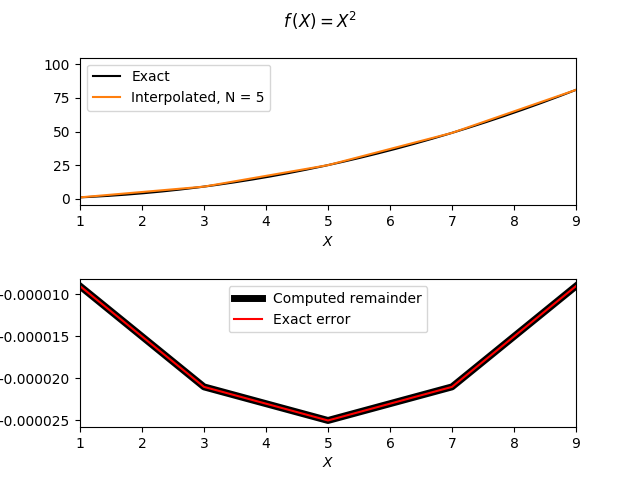
\includegraphics[scale=0.75]{LinearInterpolationError}
\end{figure}

\subsection{Mass Constant}
The mass constant, $C_{D}$, from the 3+1 GR hydrodynamics equations is:
\begin{equation}
    C_{D}\left(r\right)=\psi\left(r\right)^{6}\,\alpha\left(r\right)\,r^{2}\,\rho\left(r\right)\,W\left[v\left(r\right)\right]\,v\left(r\right).
\end{equation}
When we map from the radial coordinates from the original data to the mesh in \texttt{thornado} we don't introduce any error, because it is a linear map. This means that all the error we introduce must be due to $\rho$, $W$, and $v$. So, when deriving the error we consider the different function:
\begin{equation}
    C'_{D}\left(r\right)\equiv\f{C_{D}\left(r\right)}{\psi\left(r\right)^{6}\,\alpha\left(r\right)\,r^{2}}=\rho\left(r\right)\,W\left[v\left(r\right)\right]\,v\left(r\right).
\end{equation}

From the data we have this exact value at the two endpoints:
\begin{align}
    C'_{D}\left(r_{L}\right)&\equiv C'^{L}_{D}=\rho_{L}\,W_{L}\,v_{L}\\
    C'_{D}\left(r_{H}\right)&\equiv C'^{H}_{D}=\rho_{H}\,W_{H}\,v_{H}.
\end{align}
\newpage

\bibliographystyle{apj}
\bibliography{../References/references.bib}

\end{document}